\documentclass{jsarticle}
\usepackage[dvipdfmx]{graphicx}
\usepackage{subcaption}
\captionsetup[figure]{justification=centering}
\captionsetup[table]{justification=centering}
\usepackage[ipa]{pxchfon}

\begin{document}
\title{{\vspace*{-30mm}}{\LARGE アドバンスドコントロール課題(レポート)}}
\author{\large 千葉工業大学 先進工学部 未来ロボティクス学科 \vspace*{4mm}\\20C1015 今井悠月}
\date{}
\maketitle\vspace*{10mm}

\section*{問1}
A = [0 1; -5 -6], \hspace*{0.5zw}B = [0; 1] のシステムに対して, 最適レギュレータを設計してください.\\
\hspace*{1zw}なお, Q = [1 0; 0 1], \hspace*{0.5zw}R = 1 とします.\\
\hspace*{1zw}以下のコマンドを入力してヘルプを見ながら最適レギュレータの状態フィードバック係数ベクトルを求めて
\hspace*{1zw}ください.\vspace*{2mm}\\
\hspace*{1zw}help lqr\\

\vspace*{4mm}\subsection*{回答}
help lqr を参照の元, コードを作成し, 実行した結果は以下の図1のようになった.\\
\hspace*{1zw}講義内での手計算によって求めた結果と同様になったため, 正しく最適レギュレータを設計できたといえる.\\

\begin{figure}[htbp]
  \begin{minipage}[t]{0.5\linewidth}
    \centering
    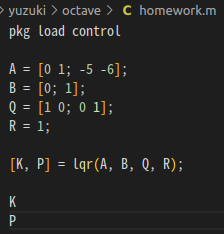
\includegraphics[keepaspectratio, scale=0.65]{fig/2.png}
    \subcaption{作成したコード}
  \end{minipage}
  \begin{minipage}[t]{0.5\linewidth}
    \centering
    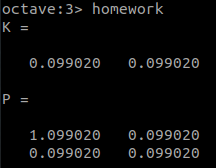
\includegraphics[keepaspectratio, scale=0.90]{fig/1.png}
    \subcaption{コード実行結果}
  \end{minipage}\vspace*{2mm}
  \caption{最適レギュレータの設計及び状態フィードバック係数ベクトルを求めるコード}
\end{figure}



\vspace*{1mm}\section*{問2}
初期値 x0 = [1; 0] として, 時間応答のグラフも求めてください.\\

\vspace*{4mm}\subsection*{回答}
上記で求めた, 最適レギュレータの状態フィードバック係数ベクトルを適用した時間応答のグラフは以下の\\
\hspace*{1zw}図2のようになった.\\

\begin{figure}[htbp]
  \begin{minipage}[t]{0.5\linewidth}
    \centering
    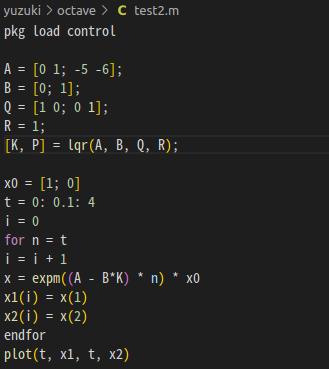
\includegraphics[keepaspectratio, scale=0.485]{fig/ato_c.png}
    \subcaption{作成したコード}
  \end{minipage}
  \begin{minipage}[t]{0.5\linewidth}
    \centering
    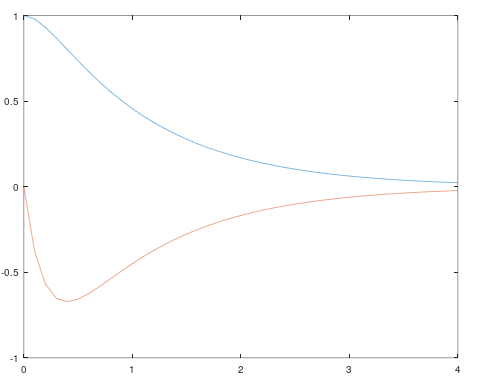
\includegraphics[keepaspectratio, scale=0.48]{fig/ato_r.png}
    \subcaption{状態フィードバック係数ベクトル適用後の\\時間応答のグラフ(コード実行結果)}
  \end{minipage}\vspace*{2mm}
  \caption{最適レギュレータの設計及び状態フィードバック係数ベクトルを求めるコード}
\end{figure}



\section*{問3}
また, Q, R をどのような値にするとより早く収束するか.\\
\hspace*{1zw}いくつか Q, R の組に対する応答を示しながら解説せよ.





% \begin{figure}[h!]
%   \centering
%    \includegraphics[height=85mm]{./figs/tukuba.png}
%    \caption{つくばチャレンジでロボットが自律移動する様子}
% \end{figure}




\end{document}
